\begin{lstlisting}
习题4.1第3,6,8题

习题4.3第6,8,9,13题
\end{lstlisting}
\begin{exercise}
设 $n\geq3$ 为无平方因子的整数,$R=\mathbb{Z}[\sqrt{ -n }]=\{ a+b:a,b\in \mathbb{Z} \}$.
	\begin{enumerate}
		\item 证明 $2,\sqrt{ -n }$ 和 $1+\sqrt{ -n }$ 在 $R$ 上均为不可约元
		\item 证明 $\sqrt{ -n }$ 和 $1+\sqrt{ -n }$ 在 $R$ 上不能同时为素元
	\end{enumerate}
\end{exercise}
\begin{example}
\begin{figure}[H]
\centering
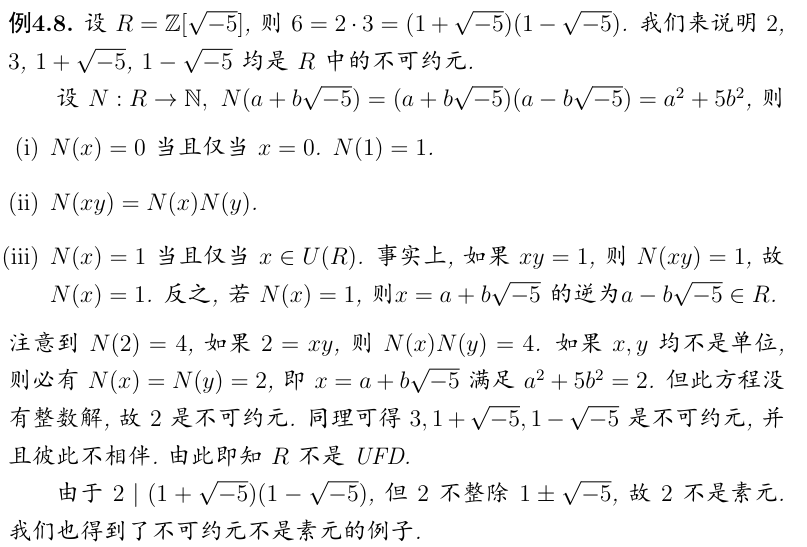
\includegraphics[width=\textwidth]{6-hw9-2025052118.png}
% \caption{}
\label{}
\end{figure}
\end{example}
The mapping
\[
\mathrm{Nm}: R\to \mathbb{Z}_{\geq 0}\qquad a+b \sqrt{ -n }\mapsto a^2+nb^2
\]
is clearly a norm. $\mathrm{Nm}(2)=4$, if $2=xy$, $x,y$ are not unit, then $x=y=2$, $x=a+b \sqrt{ -n }$ satisfies $a^2+nb^2=2$, which cannot happen. $\mathrm{Nm}(\sqrt{ -n })=n$, if $a^2+nb^2\mid n$, if $b\neq0$, then $a=0,b=\pm1$, $a+b \sqrt{ -n }=\pm\sqrt{ -n }$; thus $b=0$, $a\mid n$, but $aa'=\sqrt{ -n }$ cannot happen. $\mathrm{Nm}(1+\sqrt{ -n })=1+n$, if $a^2+nb^2\mid n+1$, if $b\neq0$, then $b=\pm1$, $a^2=1$, then $\mathrm{Nm}\left( \frac{1+\sqrt{ -n }}{a+b \sqrt{ -n }} \right)=1$, thus $\frac{1+\sqrt{ -n }}{a+b \sqrt{ -n }}$ is unit. Then $b=0$, if $1+\sqrt{ -n }$ is reducible, then $aa'=1+\sqrt{ -n }$, which cannot happen.

\begin{definition}[素元]
设$R$是一个整环,$a \in R$是一个非零非单位元,如果对任意的$b, c \in R$,若$a \mid b c$,则$a \mid b$或$a \mid c$,那么称$a$是$R$的一个\textbf{素元}.
\end{definition}
\begin{example}
证明 $\sqrt{-n}$ 和 $1+\sqrt{-n}$ 在 $R$ 上不能同时为素元。
\end{example}
我们将分两种情况讨论:$n$ 是偶数和 $n$ 是奇数。

\textbf{情况 1:$n$ 是偶数。}

由于 $n$ 是无平方因子的偶数,且 $n \geq 3$,所以 $n$ 可以写成 $n=2m$,其中 $m$ 是奇数。我们有 $\sqrt{-n} \mid n$(因为 $n=-\sqrt{-n} \cdot \sqrt{-n}$)。所以 $\sqrt{-n} \mid 2m$。如果 $\sqrt{-n}$ 是素元,那么 $\sqrt{-n} \mid 2$ 或者 $\sqrt{-n} \mid m$(即 $\sqrt{-n} \mid (n/2)$)。

\begin{itemize}
	\item $\sqrt{-n} \mid 2$ 是否可能?如果 $\sqrt{-n} \mid 2$,那么 $2=\sqrt{-n}(a+b\sqrt{-n})=a\sqrt{-n}-bn$。比较系数,我们得到 $a=0$ 且 $-bn=2$。这意味着 $n$ 整除 $2$。所以 $n=1$ 或 $n=2$。但我们已知 $n \geq 3$。因此 $\sqrt{-n}$ 不整除 $2$。(另一种方法是使用范数:如果 $\sqrt{-n} \mid 2$,则 $N(\sqrt{-n}) \mid N(2)$,即 $n \mid 4$。因为 $n$ 是偶数、无平方因子且 $n \geq 3$,所以 $n$ 不可能是 $4$ 的因子,能满足这些条件的 $n$ 不存在,$n=2$ 也被 $n \geq 3$ 排除。)
	\item $\sqrt{-n} \mid (n/2)$ 是否可能?如果 $\sqrt{-n} \mid (n/2)$,那么 $N(\sqrt{-n}) \mid N(n/2)$,即 $n \mid (n/2)^2=n^2/4$。这意味着 $1 \mid (n/4)$,所以 $4 \mid n$。但 $n$ 是无平方因子的,所以 $n$ 不能被 $4$ 整除。因此 $\sqrt{-n}$ 不整除 $n/2$。
\end{itemize}

因为 $\sqrt{-n}$ 整除乘积 $2 \cdot (n/2)$,但它既不整除 $2$ 也不整除 $n/2$,所以当 $n$ 是偶数(且 $n \geq 3$,无平方因子)时,$\sqrt{-n}$ 不是素元。

\textbf{情况 2:$n$ 是奇数。}

我们有等式 $(1+\sqrt{-n})(1-\sqrt{-n})=1-(-n)=n+1$。因为 $n$ 是奇数,所以 $n+1$ 是偶数。设 $n+1=2k$,其中 $k=(n+1)/2$ 是一个整数。于是 $(1+\sqrt{-n})(1-\sqrt{-n})=2k$。

假设 $1+\sqrt{-n}$ 是素元。

因为 $(1+\sqrt{-n}) \mid 2k$,所以 $(1+\sqrt{-n}) \mid 2$ 或者 $(1+\sqrt{-n}) \mid k$。

\begin{itemize}
	\item $(1+\sqrt{-n}) \mid 2$ 是否可能?如果 $(1+\sqrt{-n}) \mid 2$,则 $2=(1+\sqrt{-n})(a+b\sqrt{-n})$ 对某些整数 $a,b$ 成立。展开得到 $2=(a-bn)+(a+b)\sqrt{-n}$。比较系数,有 $a+b=0$(所以 $b=-a$)且 $a-bn=2$。代入 $b=-a$ 到第二个方程:$a-n(-a)=2 \Longrightarrow a(1+n)=2 \Longrightarrow a=2/(n+1)$。因为 $n$ 是奇数且 $n \geq 3$,所以 $n+1 \geq 4$。因此 $a=2/(n+1)$ 不是一个整数(因为 $0<2/(n+1)<1$)。所以 $1+\sqrt{-n}$ 不整除 $2$。
\end{itemize}

因此,如果 $1+\sqrt{-n}$ 是素元,它必须整除 $k=(n+1)/2$。这意味着 $(n+1)/2=(1+\sqrt{-n})(c+d\sqrt{-n})$ 对某些整数 $c,d$ 成立。将此代入原方程 $(1+\sqrt{-n})(1-\sqrt{-n})=2k$:$(1+\sqrt{-n})(1-\sqrt{-n})=2(1+\sqrt{-n})(c+d\sqrt{-n})$。因为 $N(1+\sqrt{-n})=n+1 \neq 0$,所以 $1+\sqrt{-n} \neq 0$。由于 $R$ 是一个整环(integral domain),我们可以消去 $1+\sqrt{-n}$:$1-\sqrt{-n}=2(c+d\sqrt{-n})$。这意味着 $2 \mid (1-\sqrt{-n})$。所以 $1-\sqrt{-n}=2c+2d\sqrt{-n}$。比较系数:$1=2c$ 且 $-1=2d$。这对于整数 $c,d$ 是不可能的。

这个矛盾表明,如果 $n$ 是奇数(且 $n \geq 3$,无平方因子),那么 $1+\sqrt{-n}$ 不是素元。

\begin{exercise}
设 $R$ 是整环. 证明多项式环 $R[x]$ 是 PID 当且仅当 $R$ 是域.
\end{exercise}
若 $R$ 为域,那么存在 $\mathrm{Nm}:R[x]\to \mathbb{Z}_{\geq0},f(x)\mapsto \deg f$, 故 $R[x]$ 是 ED,故为 PID. 若 $R[x]$ 为 PID,那么对任意理想 $(a)\subset R$,考虑理想 $(a,x)\subset R[x]$,由于 $R[x]$ 是 PID,故存在 $h (x)\in R[x]$ 使得 $(a,x)=(h(x))$. 由于 $h(x)\mid a$,故 $\deg h=0$,$h=c\in R$,由于 $c\mid x$,故 $c\mid1$ 为单位元. $(a,x)=(1)$,由于 $1\in(a,x)$,故 $aa'=1$,$a$ 是单位,故 $(a)=(1)$. $R$ 的任意理想平凡,故 $R$ 是域.

\begin{exercise}
\begin{figure}[H]
\centering
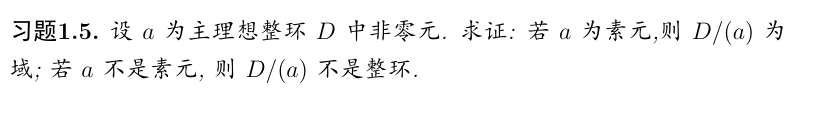
\includegraphics[width=\textwidth]{5-hw9-2025052118.png}
% \caption{}
\label{}
\end{figure}
\end{exercise}
在 PID 中,素理想都是极大理想,故 $D/(a)$ 为域.

$a$ 是素元当且仅当 $(a)$ 是素理想,当且仅当 $D/(a)$ 是整环.

\begin{exercise}
\begin{figure}[H]
\centering

\includegraphics[width=\textwidth]{1-hw9-2025052118.png}
% \caption{}
\label{}
\end{figure}
\end{exercise}
反证而设 $\alpha+\beta\in \mathbb{Q}$, 记 $g(x)=f\left( x+\frac{\alpha+\beta}{2} \right),h(x)=g(x)+g(-x)$. 若 $h\neq0$, 则
\[
h\left( \frac{\beta-\alpha}{2} \right)=f(\alpha)+f(\beta)=0=g\left( \frac{\beta-\alpha}{2} \right)
\]
于是 $\deg(\gcd(g,h))\geq1$, 由于 $\deg g$ 为奇数,$\deg h$ 为偶数,故 $\deg(\gcd(g,h))\leq \deg h<\deg g$,于是 $\gcd(g,h)$ 是 $g$ 的非平凡因子,这与 $g$ 不可约矛盾. 故 $h=0$, $g$ 的 $x^{2k}$ 前系数为 0,$k\geq0$,于是 $x\mid g$,这与 $g$ 不可约矛盾.

\begin{exercise}
\begin{figure}[H]
\centering

\includegraphics[width=\textwidth]{2-hw9-2025052118.png}
% \caption{}
\label{}
\end{figure}
\end{exercise}
$\mathbb{R}[x]$ 是 PID, $\mathbb{R}[x]$ 的不可约元为一次多项式、无实根的二次多项式,$(x-c)$ 或 $(x-a)^2+b^2$. 于是 $\mathbb{R}[x]$ 的所有素理想(即极大理想)为 $\left< 0 \right>$, $\left< x-c \right>$,$\left< (x-a)^2+b^2 \right>$, 其中 $a, b, c\in \mathbb{R}$.

$\mathbb{Z}[x]$的素理想总结:

\begin{enumerate}
	\item $\langle 0\rangle$ (零理想)。
	\item $\langle p\rangle$, 其中$p$ 是$\mathbb{Z}$ 中的素数。
	\item $\langle f(x)\rangle$, 其中$f(x)$ 是$\mathbb{Z}[x]$ 中的非零本原不可约多项式。
	\item $\langle p,f(x)\rangle$, 其中$p$ 是$\mathbb{Z}$ 中的素数,$f(x)\in\mathbb{Z}[x]$ 且其系数模$p$ 后得到的$\overline{f}(x)\in\mathbb{Z}_p[x]$ 是$\mathbb{Z}_p[x]$ 中的不可约多项式。
\end{enumerate}

$\mathbb{Z}[x]$的极大理想总结:

$\mathbb{Z}[x]$ 中的极大理想只有上述第 4 类理想:

$\langle p,f(x)\rangle$, 其中$p$ 是$\mathbb{Z}$ 中的素数,$f(x)\in\mathbb{Z}[x]$ 且其系数模$p$ 后得到的$\overline{f}(x)\in\mathbb{Z}_p[x]$ 是$\mathbb{Z}_p[x]$ 中的不可约多项式。好的,我们来确定$\mathbb{R}[x]$ 和$\mathbb{Z}[x]$ 的所有素理想和极大理想。

\begin{exercise}
\begin{figure}[H]
\centering

\includegraphics[width=\textwidth]{3-hw9-2025052118.png}
% \caption{}
\label{}
\end{figure}
\end{exercise}
\begin{figure}[H]
\centering
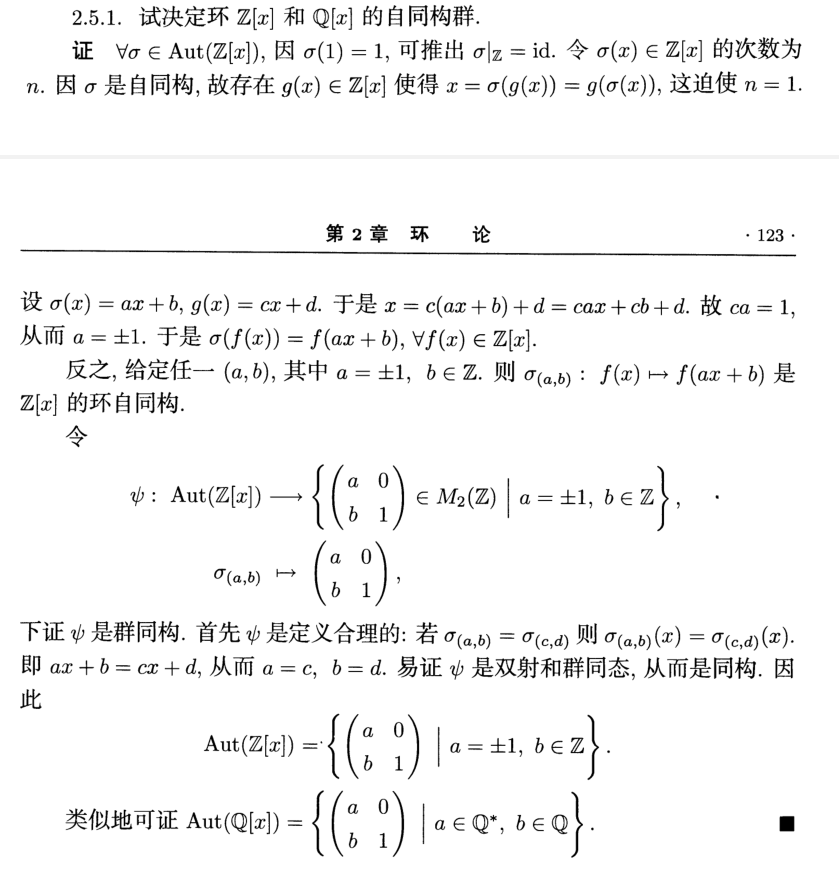
\includegraphics[width=\textwidth]{hw9-2025052200.png}
% \caption{}
\label{}
\end{figure}

\begin{exercise}
\begin{figure}[H]
\centering

\includegraphics[width=\textwidth]{4-hw9-2025052118.png}
% \caption{}
\label{}
\end{figure}
\end{exercise}
若 $f(x)=g(x)h(x)$, $1\leq \deg g,\deg h<\deg f$, $g, h\in F[x]$,则 $f(ax+b)=\widetilde{g}(x)\widetilde{h}(x)$, 其中 $\widetilde{g}(x)\coloneqq g (ax+b)\in F[x]$, $\widetilde{h}(x)=h (ax+b)\in F[x]$. 反之,若 $f(ax+b)\eqqcolon\widetilde{f}(x)$ 可约,将前面的推导应用到 $\widetilde{f}\left( \frac{1}{a}(x-b) \right)$ 上,就有 $f(x)$ 可约. 故 $f(x)$ 在 $F[x]$ 中可约当且仅当 $f(ax+b)$ 在 $F[x]$ 中可约. 故 $f(x)$ 在 $F[x]$ 中不可约当且仅当 $f(ax+b)$ 在 $F[x]$ 中不可约.
